\documentclass{beamer}

\usepackage[ngerman]{babel}
\usepackage{graphicx} % fuer Bilder
\usepackage{listings} % fuer Code
\usepackage{lmodern}

%\usetheme{Goettingen}

%% Formatierung des Sourcecodes
\DeclareFontShape{OT1}{cmtt}{bx}{n}{<5><6><7><8><9><10><10.95><12><14.4><17.28><20.74><24.88>cmttb10}{}
\definecolor{eclipse-violet}{rgb}{0.50, 0.0, 0.46}
\definecolor{eclipse-green}{rgb}{0.25, 0.50, 0.37}
\definecolor{eclipse-blue}{rgb}{0.17, 0.0, 1.00}
\lstset{
 language=C++, % fuer c++ code style
 showstringspaces=false,
 basicstyle=\ttfamily\small,
 keywordstyle=\bfseries\color{eclipse-violet},
 commentstyle=\color{eclipse-green},
 stringstyle=\color{eclipse-blue}
}

\title{Prozesslenkung: Hierarchische Zustandsautomaten II}
\subtitle{Implementierung Hierarchischer Zustandsautomaten}
\author{Katja Kirstein, Anne-Lena Kowalka, Marian Triebe, Eugen Winter}
\date{\today}

\begin{document}

\begin{frame}
 \titlepage
\end{frame}

%% Themen uebersicht
\begin{frame}
 \frametitle{Themen}
 \begin{itemize}
  \item Implementierungs Arten
  \item Externe Statevariablen
  \item Guards
  \item Entry und Exit Code
  \item History
  \item Timer
 \end{itemize}
\end{frame}

%% Beispiel
\begin{frame}
 \frametitle{Beispiel F\"orderband}
 \begin{center}
   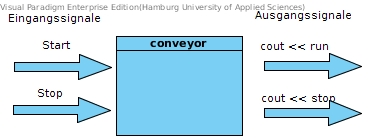
\includegraphics[scale=.5]{img/Systemgrenzen_fsm_gof.jpg}
   \newline
  \end{center}
  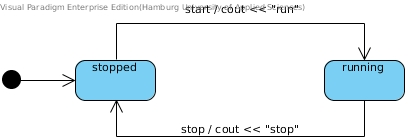
\includegraphics[scale=.6]{img/fsm_gof_automat.jpg}
\end{frame}

%% Switch Case Implementierung 1
\begin{frame}
  \frametitle{Geschachtelte Switch-Case-Anweisung}
  \begin{itemize}
    \item Zust\"ande und Signale werden durch enums repr\"asentiert
    \item der aktuelle Zustand wird durch Zustandsvariable repr\"asentiert
    \item 2-Level-Switch Case erforderlich: 1. Level pr\"uft aktuellen Zustand,
    2. Level pr\"uft erhaltenes Signal
    \item es empfiehlt sich, den Automaten in einer dispatch-Methode zu kapseln
  \end{itemize}
\end{frame}

%% Switch Case Implementierung 2
\begin{frame}[fragile]
  \frametitle{Beispiel der dispatch-Methode}
  \begin{lstlisting}
enum State{ srunning, sstopped }; // Zustaende

enum Signal{ Start, Stop }; //Eingangssignale

void dispatch(Signal sig){
  switch(state){ // Zustand pruefen
    case srunning:
      switch(sig){ // erhaltenes Signal pruefen
        case Start: // bereits srunning  
          break; // -> keine Reaktion erforderlich
        case Stop:
          tran(sstopped); //Transition
          stopped(); //cout << "stop"<<endl;
          break;
      }
    // ...
  }  
};
  \end{lstlisting}
\end{frame}

%% Switch Case Implementierung 3
\begin{frame}
  \frametitle{Vor- und Nachteile geschachtelter Switch-Case-Automaten}
  \begin{itemize}
    \item Vorteile:
    \begin{itemize}
      \item einfach und leicht verst\"andlich
      \item wenig Speicher ben\"otigt (nur eine State-Variable)
    \end{itemize}
    \item Nachteile
    \begin{itemize}
      \item die Verarbeitungszeit h\"angt von der Anzahl von Zust\"anden und Signalen ab
      \item die Umsetzung hierarchischer Automaten ist schwierig 
    \end{itemize}
  \end{itemize}
\end{frame}

%% Switch Case Implementierung 1 ungeschachtelt
\begin{frame}
  \frametitle{Implementierung II : Ungeschachtelte Switch-Case-Anweisung nach Samek}
  \begin{itemize}
    \item Zust\"ande werden durch typedef einer Pointer-to-Member-Funktion mit Signal als Parameter repr\"asentiert (  typedef void (Kontext::*State)(unsigned const sig);  )
    \item die dispatch-Methode \"ubergibt das erhaltene Signal an diese State-Variable (bzw. die Pointer-to-Member-Funktion) 
    \item die Zust\"ande werten die Signale dann mittels switch-case aus
  \end{itemize}
\end{frame}

%% Switch Case Implementierung 2 ungeschachtelt
\begin{frame}[fragile]
  \frametitle{Beispiel einer Pointer-to-Member-Funktion}
  \begin{lstlisting}
enum Signal{ Start, Stop }; //Eingangssignale
//...
void dispatch(unsigned const sig) {
  this->*myState) (sig); } 
//...
void Kontext::running(Signal sig){
  switch(sig){ //im Zustand running erhaltenes Signal pruefen
    case Start: // da bereits srunning  ..
    break; // ..-> keine Reaktion erforderlich
  case Stop:
    tran(sstopped); //Transition
    stopped(); //cout << "stop"<<endl;
    break;
  }
}  
  \end{lstlisting}
\end{frame}

%% Switch Case Implementierung 3 ungeschachtelt
\begin{frame}
  \frametitle{Vor- und Nachteile ungeschachtelter Switch-Case-Automaten}
  \begin{itemize}
    \item Vorteile:
    \begin{itemize}
      \item leicht verst\"andliche Struktur/ einfache Umsetzung
      \item speicherschonend, da nur der state-Pointer gespeichert werden muss
      \item Code kann wiederverwendet werden, da der generische Teil (init, dispatch und tran-Methoden) in einer Klasse gekapselt werden kann
      \item effizient, da ein switch-case-Level wegf\"allt
      \item \"Anderungen im Automaten sind leicht umsetzbar
    \end{itemize}
    \item Nachteile
    \begin{itemize}
      \item die verbliebene Switch-Case-Anweisung ist immernoch von der Anzahl Signale abg\"angig
      \item nicht f\"ur hierarchische Automaten geeignet
    \end{itemize}
  \end{itemize}
\end{frame}

%% State Table
\begin{frame}
 \frametitle{Zustandstabelle}
 Am Beispiel des F\"orderbands
 \newline
 \begin{center}
 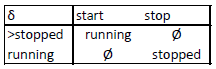
\includegraphics{img/zustandstabelle.PNG}
 \end{center}
\end{frame}

%% State Table Implementierung I
\begin{frame}[fragile]
 \frametitle{Zustandstablle Implementierung I}
 \begin{lstlisting}
// Zustaende
enum states {
  STOPPED,
  RUNNING,
};

// Eingangssignale
enum input {
  START,
  STOP
};

struct transition {
  states m_state;
  input  m_input;
  states m_next;
  void (*m_fn) (void); // Funktionspointer
};
 \end{lstlisting}
\end{frame}

%% State Table Implementierung II
\begin{frame}[fragile]
 \frametitle{Zustandstablle Implementierung II}
 \begin{lstlisting}
// Context Klasse
class conveyor {
  static void starten();
  static void stoppen();
  // Transitionstabelle
  static transition trans[];
  // aktueller Zustand
  states m_state;
 public:
  void do_action(input in);
  conveyor() : m_state(STOPPED) { }
};
 \end{lstlisting}
 Initialisierung des Zustandsarrays
 \begin{lstlisting}
transition conveyor::trans[] = {
  { STOPPED, START, RUNNING, &conveyor::starten },
  { RUNNING, STOP,  STOPPED, &conveyor::stoppen }
};
 \end{lstlisting}
\end{frame}

%% State Table Implementierung III
\begin{frame}[fragile]
 \frametitle{Zustandstablle Implementierung III}
 \"Ubergangsfunktion in der Context Klasse
 \begin{lstlisting}
void conveyor::do_action(input in) {
  for (int i = 0; i < TRANS_COUNT; ++i) {
    if (trans[i].m_state == this->m_state &&
        trans[i].m_input == in) {
      trans[i].m_fn();
      // Zustandswechsel
      this->m_state = trans[i].m_next;
      return;
    }
  }
  // Fehlerausgabe hier moeglich
  std::cout << "no action" << std::endl;
}
 \end{lstlisting}
\end{frame}

%% Vor- und Nachteile Zustandstabelle
\begin{frame}
 \frametitle{Vor- und Nachteile Zustandstablle}
 \begin{itemize}
  \item Vorteile:
  \begin{itemize}
   \item Einfach zu Implementieren
   \item Keine NOP Operationen/Funktionen notwenig
   \item Tabelle hat nur so viele Eintr\"age wie \"Uberg\"ange
  \end{itemize}
  \item Nachteil:
  \begin{itemize}
   \item Langsamer Zugriff
  \end{itemize}
 \end{itemize}
\end{frame}

%% Matrix Implementierung I
\begin{frame}[fragile]
 \frametitle{Zustandsmatrix Implementierung I}
 \begin{lstlisting}
// Zustaende
enum states {
  NO_CHANGE = -1,
  STOPPED,  // 0
  RUNNING,  // 1
};

// Eingangssignale
enum input {
  START, // 0
  STOP   // 1
};

// Ein Eintrag in der Tabelle
struct transition {
  states m_next;
  void (*m_fn) (void); // Funktionspointer
};
 \end{lstlisting}
\end{frame}

%% Matrix Implementierung II
\begin{frame}
 \frametitle{Zustandsmatrix Implementierung II}
 \begin{itemize}
  \item Deklaration in der Context Klasse ist nun ein 2 Dimmensionales Array!
 \end{itemize}
 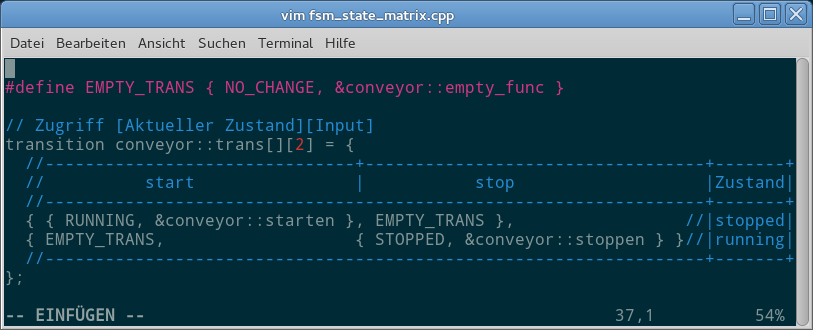
\includegraphics[scale=.4]{img/matrix_vim.png}
\end{frame}

%% Matrix Implementierung III
\begin{frame}[fragile]
 \frametitle{Zustandsmatrix Implementierung III}
 \"Ubergangsfunktion in der Context Klasse
 \begin{lstlisting}
void conveyor::do_action(input in) {
  int dim1 = static_cast<int>(this->m_state);
  int dim2 = static_cast<int>(in);
  trans[dim1][dim2].m_fn();
  if (trans[dim1][dim2].m_next != NO_CHANGE) {
    this->m_state = trans[dim1][dim2].m_next;
  }
}
 \end{lstlisting}
\end{frame}

%% Vor- und Nachteile Zustandstabelle
\begin{frame}
 \frametitle{Vor- und Nachteile Zustandstablle}
 \begin{itemize}
  \item Vorteile:
  \begin{itemize}
   \item Gute Performance
   \item Weniger Speicherverbrauch pro Eintrag
  \end{itemize}
  \item Nachteil:
  \begin{itemize}
   \item Schwerer zu implementieren
   \item Matrix ben\"otigt insgesamt mehr Speicher da alle F\"alle auskodiert werden m\"ussen
   \item NOP Funktion ben\"otigt
  \end{itemize}
 \end{itemize}
\end{frame}

%% GoF fsm Beispiel (Klassendiagramm)
\begin{frame}
 \frametitle{GoF State Pattern Struktur}
 \begin{center}
   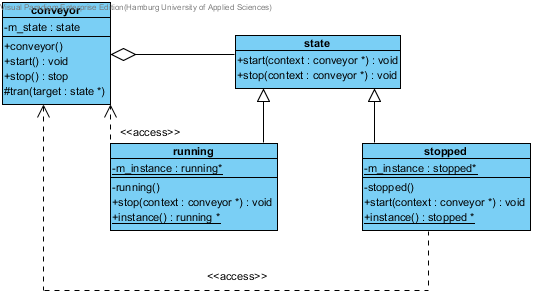
\includegraphics[scale=.65]{img/GoF_pure.png}
 \end{center}
 \begin{itemize}
  \item Kontext-Klasse (conveyor)
  \item Zustands Basisklasse (state)
  \item Zust\"ande (running, stopped)
 \end{itemize}
\end{frame}

%% GoF fsm pure
\begin{frame}[fragile]
 \frametitle{GoF Implementierung I Header}
 \begin{lstlisting}
class conveyor {
  friend class stopped;
  friend class running;
 public:
  conveyor(): m_state(stopped::instance()) { }
  void start();
  void stop();
 private:
  state* m_state;
 protected:
  void tran(state* target);
};
 \end{lstlisting}
\end{frame}

%% GoF fsm pure
\begin{frame}[fragile]
 \frametitle{GoF Implementierung II Header}
 \begin{lstlisting}
class running : public state {
  static running* m_instance;
 public:
  void stop(conveyor* context);
  static running* instance() {
    if (!m_instance) {
      m_instance = new running();
    }
    return m_instance;
  }
 private:
  running() { };
};
 \end{lstlisting}
\end{frame}

%% GoF fsm pure
\begin{frame}[fragile]
 \frametitle{GoF Implementierung III}
 \begin{lstlisting}
// Zustandswechsel funktion
void conveyor::tran(state* target) {
  m_state = target;
}

// transition running -> stopped
void running::stop(conveyor* context) {
  cout << "running: stop()" << endl;
  context->tran(stopped::instance());
}
 \end{lstlisting}
\end{frame}


%% Grundlagen GoF
\begin{frame}
 \frametitle{Grundlagen GoF}
 Die klassiche GoF Implementierung hat einige schw\"achen
 \begin{itemize}
  \item Hoher Speicherverbrauch, da jeder Zustand im Speicher gehalten werden muss, auch wenn diese eigentlich nicht verwendet werden
  \item Der h\"ohere Speicherverbrauch kann allerdings mit dem Placement New Operator umgangen werden
  \item Kontext muss eventuell immer mit \"ubergeben werden
 \end{itemize}
\end{frame}

%% GoF fsm Systemgrenzen
\begin{frame}
 \frametitle{GoF nach Pareigis/Manske}
 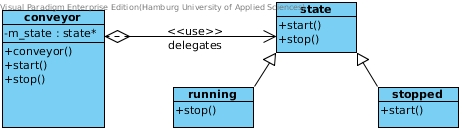
\includegraphics[scale=.6]{img/fsm_gof.jpg}
\end{frame}

%% GoF fsm States in Code I
\begin{frame}
 \frametitle{GoF States in Code I}
 \begin{itemize}
  \item Alle States erben von einer Oberstate Klasse
  \item Der Oberstate implementiert alle Events aller Zust\"ande als leere virtuelle Funktion
  \item Der jeweilige Zustand implementiert nur seine eigenen Events, nicht relevante
  Events werden an die leeren Methoden der Basisklasse weitergereicht
 \end{itemize}
\end{frame}

%% GoF fsm States in Code (Header)
\begin{frame}[fragile]
 \frametitle{GoF States in Code (Header)}
 \begin{lstlisting}
class state {
 public:
  virtual ~state() { }
  virtual void start() { }
  virtual void stop() { }
};

class running : public state {
 public:
  void stop();
};

class stopped : public state {
 public:
  void start();
};
 \end{lstlisting}
\end{frame}

%% GoF fsm States in Code (Implementierung/CPP)
\begin{frame}[fragile]
 \frametitle{GoF States in Code (Implementierung)}
 \begin{lstlisting}
// transition running -> stopped
void running::stop() {
  new (this) stopped;
  cout << "stop() / stop" << endl;
}

// transition stopped -> running
void stopped::start() {
  new (this) running;
  cout << "start() / run" << endl;
}
 \end{lstlisting}
\end{frame}

%% GoF fsm Kontext Klasse
\begin{frame}
 \frametitle{GoF Kontext Klasse}
 \begin{itemize}
  \item Sicht von au{\ss}en auf die FSM
  \item Dient als Delegator zu den Zust\"anden
  \item Bedient alle Eingangssignale durch Funktionen
 \end{itemize}
\end{frame}

%% GoF fsm Konext Klasse
\begin{frame}[fragile]
 \frametitle{GoF Kontext Klasse in Code}
 Header:
 \begin{lstlisting}
class conveyor {
 public:
  conveyor() : m_state(new stopped) { }
  ~conveyor() { delete m_state; }
  void start();
  void stop();
 private:
  state* m_state;
};
 \end{lstlisting}
 Implementierung:
 \begin{lstlisting}
void conveyor::start() {
  m_state->start();
}

void conveyor::stop() {
  m_state->stop();
}
 \end{lstlisting}
\end{frame}

%% Schritte zum erstellen einer FSM
\begin{frame}
 \frametitle{Schritte zum erstellen einer FSM}
 \begin{enumerate}
  \item Erstellen der Systemgrenzen
  \item Erstellen einer FSM
  \item Umwandlung in Code
  \begin{itemize}
   \item Kontextklasse, Funktionsnamen als Eingangssignale
   \item Basisklasse f\"ur Zust\"ande erstellen
   \item Zustandsklassen erben von der Basisklasse und implementieren nur die eigenen Reaktionen neu
  \end{itemize}
  \item Pr\"ufen ob Code und Systemgrenzen/Diagramm zusammenpassen
  \begin{itemize}
   \item Sind alle Eingangssignale als Funktionen zu finden?
   \item Werden alle Ausgangssignale verwendet/ausgegeben?
   \item Die Namen f\"ur Eingangssignale/Ausgangssignale sollten konsistent sein, da Fehler sonst vorprogrammiert!
  \end{itemize}
 \end{enumerate}
\end{frame}

%% Übung GoF
\begin{frame}
 \frametitle{\"Ubung Lichtschalter}
 Erstellt die Systemgrenzen, Automatendiagramm, und Code eines Lichtschalters (An und Aus Button). (15 Min)
\end{frame}

%% Orthogonale Automaten
\begin{frame}
 \frametitle{Orthogonale Automaten}
 \begin{itemize}
  \item Alle Automaten bekommen das Eingangssignal
  \item Nur die betreffende Instanz reagiert
 \end{itemize}
\end{frame}


%% Externe Statevariablen
\begin{frame}
 \frametitle{Externe Statevariablen}
 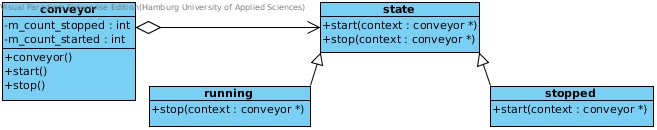
\includegraphics[scale=.44]{img/fsm_externe_state_var.jpg}
\end{frame}

%% Implementierung von externen Statevariablen I
\begin{frame}[fragile]
 \frametitle{Implementierung von externen Statevariablen I}
 \begin{lstlisting}
class conveyor {
  friend class running;
  friend class stopped;
 public:
  conveyor()
      : m_state(new stopped),
        m_count_stopped(0),
        m_count_started(0) { }
  ~conveyor() { delete m_state; }
  void start();
  void stop();
 private:
  state* m_state;
  int m_count_stopped;
  int m_count_started;
};
\end{lstlisting}
\end{frame}

%% Implementierung von externen Statevariablen II
\begin{frame}[fragile]
 \frametitle{Implementierung von externen Statevariablen II}
 Header:
 \begin{lstlisting}
class state {
 public:
  virtual ~state() { }
  virtual void start(conveyor* context) { }
  virtual void stop(conveyor* context) { }
};

class running : public state {
 public:
  void stop(conveyor* context);
};

class stopped : public state {
 public:
  void start(conveyor* context);
};
 \end{lstlisting}
\end{frame}

%% Implementierung von externen Statevariablen III
\begin{frame}[fragile]
 \frametitle{Implementierung von externen Statevariablen III}
 Implementierung:
 \begin{lstlisting}
// transition stopped -> running
void stopped::start(conveyor* context) {
  ++context->m_count_started;
  new (this) running;
}

void conveyor::start() {
  m_state->start(this);
}
 \end{lstlisting}
\end{frame}

%% Guards
\begin{frame}
 \frametitle{Guards}
 \begin{center}
   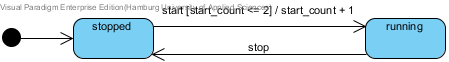
\includegraphics[scale=.8]{img/fsm_gof_guard_automat.png}
 \end{center}
\end{frame}

%% Guard Implementierung
\begin{frame}[fragile]
 \frametitle{Guards Implementierung}
 Implementierung:
 \begin{lstlisting}
// transition stopped -> running
void stopped::start(conveyor* context) {

  ++context->m_count_started;

  if (context->m_count_started <= 2) {
    new (this) running;
  } else {
    return;
  }
}
 \end{lstlisting}
\end{frame}

%% �bung Guards
\begin{frame}
 \frametitle{\"Ubung Lichtschalter II}
 Implementieren sie einen Lichtschalter der nach mehrfachem bet\"atigen der Starttaste in ein anderes Licht wechselt
\end{frame}

%% Entry/Exit Code 1
\begin{frame}
 \frametitle{Entry/Exit Code in HSM }
 \begin{itemize}
  \item Zustandswechsel d\"urfen Hierarchieebenen nicht \"uberspringen
  \item exit() wird durchgef\"uhrt, wenn Signale in der Hierarchie "nach oben" weitergereicht werden
  \item entry() wird  durchgef\"uhrt, wenn Signale in der Hierarchie "nach unten" weitergereicht werden
 \end{itemize}
\end{frame}

%% Entry/Exit Code 2
\begin{frame}
 \frametitle{Entry/Exit Code in HSM }
 \begin{itemize}
  \item Beispiel exit: State S12 erh\"alt Signal e\newline\newline
  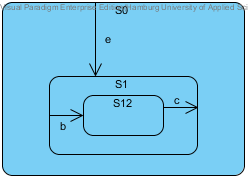
\includegraphics[scale=.8]{img/beispiel_exitSM}
 \end{itemize}
\end{frame}

%% Exit Code 3
\begin{frame}[fragile]
 \frametitle{Entry/Exit Code in HSM }
 \begin{lstlisting}
 //State S12 erhaelt Signal e
 void StateS12::sigE() {
   exit();
   new (this) StateS1;
   sigE();
 }
 \end{lstlisting}
 \begin{itemize}
  \item die exit-Funktion ist in jedem Zustand definiert
  \item wenn auch der Top-Zustand nicht auf ein Signal reagiert, sollte dieser z.B. eine
  failure-Methode haben, um den Fehler anzuzeigen
 \end{itemize}
\end{frame}

%% Entry Code 1
\begin{frame}
 \frametitle{Entry/Exit Code in HSM  }
 \begin{itemize}
  \item Beispiel entry: State S1 erh\"alt Signal b\newline\newline
  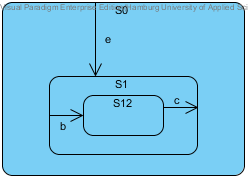
\includegraphics[scale=.8]{img/beispiel_exitSM}
 \end{itemize}
\end{frame}

%% Entry Code 2
\begin{frame}[fragile]
 \frametitle{Entry/Exit Code in HSM }
 \begin{lstlisting}
//State S1 erhaelt Signal b
void StateS1::init(T* t) {

  //t ist ein Pointer auf die Kontextklasse
  void* history = t->getStateFromHistory(StateS1ID);

  if(history != 0) {
    memcpy(this, &history, 4);
  } else {
    new (this) StateS12;
    entry();
  }
  init();
}
 \end{lstlisting}
\end{frame}

%% Entry Code 3
\begin{frame}[fragile]
 \begin{itemize}
  \item die entry-Funktion ist in jedem Zustand definiert
  \item init() f\"uhrt dazu, dass -sofern ein Substate bereits in der History vorliegt- dieser direkt betreten wird; ansonsten wird er neu erzeugt
  \item die init()-Funktion in der letzten Ebene ist leer
 \end{itemize}
\end{frame}

%% History 1
\begin{frame}
 \frametitle{History}
 \begin{itemize}
  \item Implementierung der flachen History
  \item die history-Funktion  wird in der exit-Funktion aufgerufen
  \item die Kontextklasse h\"alt ein History- Array,
  in dem sich die Subzust\"ande mittels history-Aufruf eintragen (Index-Zuordnung z.B. \"uber enums)
 \end{itemize}
\end{frame}

%% History 2
\begin{frame}[fragile]
 \frametitle{History}
 \begin{itemize}
  \item Beispiel: S1 tr\"agt sich in History-Tabelle ein
 \end{itemize}
 \begin{lstlisting}
//StateS1 history-Funktion
voidS StateS1::history(T* t) {
  //t ist ein Pointer auf die Kontextklasse
  t->setHistory(State::StateID::StateS1_ID,
                this);
}
 \end{lstlisting}
 \begin{itemize}
  \item der Parameter StateS1ID gibt den Index in der History-Tabelle in der Kontextklasse an
 \end{itemize}
\end{frame}

%% History 3
\begin{frame}[fragile]
 \frametitle{History}
 \begin{itemize}
  \item setHistory in der Kontextklasse:
 \end{itemize}
 \begin{lstlisting}
  void setHistory(int ID, State* ptr) {
    history_[ID] = *((void**) ptr);
  }
 \end{lstlisting}
 \begin{itemize}
  \item ptr wird zun\"achst auf void** gecastet, damit man mit einer weiteren Dereferenzierung * an die virtuelle Funktionstabelle des Zustands gelangt
 \end{itemize}
\end{frame}

%% History 4
\begin{frame}[fragile]
 \frametitle{History}
 \begin{itemize}
  \item getStateFromHistory in der Kontextklasse:
 \end{itemize}
 \begin{lstlisting}
  void* getStateFromHistory(int ID) {
    return history_[ID];
  }
 \end{lstlisting}
 \begin{itemize}
  \item \"uber seine ID kann der Zustand sich seine History -sofern eine vorliegt- aus der History-Tabelle in der Kontextklasse holen
 \end{itemize}
\end{frame}

%% Timer 1
\begin{frame}[fragile]
 \frametitle{Timer}
 \begin{itemize}
  \item Definition der Zeit-Messung eines Timers:\newline\newline
  $\bullet$ \textbf{Absolut}: L\"ose aus \textbf{am} 24.12.2014\newline
  (Zeit vergangen seit 01.01.1970 00:00)\newline\newline
  $\bullet$ \textbf{Relativ}: L\"ose aus \textbf{in} 10 Sekunden\newline
  (Zeit vergangen seit Start des Timers)
 \end{itemize}
\end{frame}

%% Timer 2
\begin{frame}[fragile]
 \frametitle{Timer}
 \begin{itemize}
  \item Definition des Zeit-Intervalls eines Timers:\newline\newline
  $\bullet$ \textbf{Periodisch}: L\"ose alle 100 Millisekunden aus\newline\newline
  $\bullet$ \textbf{One-Shot}: L\"ose einmalig in 10 Sekunden aus
 \end{itemize}
\end{frame}

%% Timer 3
\begin{frame}[fragile]
 \frametitle{Timer}
 \begin{itemize}
  \item Ereignis beim Ausl\"osen eines Timers:\newline\newline
  $\bullet$ \textbf{Pulse Message}: Sende eine Pulse Message\newline\newline
  $\bullet$ \textbf{Signal senden}: Sende ein Signal (z.B. SIGTERM)\newline\newline
  $\bullet$ \textbf{Thread starten}: Starte einen bestimmten Thread
 \end{itemize}
\end{frame}

%% Timer 4
\begin{frame}[fragile]
 \frametitle{Timer}
 \begin{itemize}
  \item Erforderliche Schritte f\"ur die Nutzung eines Timers:\newline\newline
  \textbf{1.} Timer Objekt erstellen\newline\newline
  \textbf{2.} Entscheiden, wie man benachrichtigt werden m\"ochte (Pulse Message, Signal, Thread) und dementsprechend das \textbf{struct sigevent} initialisieren\newline\newline
  \textbf{3.} Entscheiden, welche Art von Timer man w\"ahlt (relativ vs. absolut \& one-shot vs. periodisch)\newline\newline
  \textbf{4.} Timer starten
 \end{itemize}
\end{frame}

%% Timer 5
\begin{frame}[fragile]
 \frametitle{Timer}
 Beispiel f\"ur die Erstellung eines Timers (1/2):
 \begin{lstlisting}
// 1.
timer_t timerid;
struct sigevent event;
struct itimerspec timer;

// 2.
SIGEV_PULSE_INIT(
  &event, // struct sigevent
  coid,   // Connection ID of message receiver
  SIGEV_PULSE_PRIO_INHERIT, // Priority
  MY_CODE_TIMER, // Code for pulse handler
  MY_VALUE_TIMER // Value for pulse handler
);
 \end{lstlisting}
\end{frame}

%% Timer 6
\begin{frame}[fragile]
 \frametitle{Timer}
 Beispiel f\"ur die Erstellung eines Timers (2/2):
 \begin{lstlisting}
// 3. Create timer with realtime clock
timer_create(CLOCK_REALTIME, &event, &timerid);

// Setup the timer (2s delay, 1s reload)
// it_value = one-shot value
// it_interval = reload value
timer.it_value.tv_sec = 2;
timer.it_value.tv_nsec = 0;
timer.it_interval.tv_sec = 1;
timer.it_interval.tv_nsec = 0;

// 4. Start the timer
timer_settime(timerid, 0, &timer, NULL);
 \end{lstlisting}
\end{frame}

%% Timer 7
\begin{frame}[fragile]
 \frametitle{Timer}
 \begin{itemize}
  \item Hinweis f\"ur die Abfrage des Benachrichtigung-Typs:\newline
  \begin{lstlisting}
// Don't read the struct sigevent directly
if(event.sigev_notify == SIGEV_PULSE)

// Use this macro instead
if(SIGEV_GET_TYPE(&event) == SIGEV_PULSE)
  \end{lstlisting}
 \end{itemize}
\end{frame}

%% Timer 8
\begin{frame}[fragile]
 \frametitle{Timer}
 \begin{itemize}
  \item TODO:\newline\newline
  $\bullet$ \textbf{BEISPIEL}: Server, der auf Timer / Clients wartet\newline\newline
  $\bullet$ \textbf{BEISPIEL}: Orthogonale Automaten\newline\newline
 \end{itemize}
\end{frame}

%% Prüfungsfragen
\begin{frame}
 \frametitle{Pr\"ufungsfragen}
 \begin{itemize}
  \item Welche Arten von Implementierungen gibt es?
  \item Wie geht man Schrittweise vor einen Automaten zu implementieren?
  \item Was ist zu beachten bei Statevariablen und die Nachteile die dadurch entstehen?
  \item Wie geht man vor einen Timer zu implementieren?
 \end{itemize}
\end{frame}

\end{document}
